% =====================================================================
%  ch09.tex —— 第 9 章 有限群的分类空间与群上同调（原书 p.130–141 页首）
%  §9.1 分类空间 $BG$ 的构造  §9.2 $BG$ 的单纯上同调
%  §9.3 $H^2$ 与群扩张  §9.4 $H^3$ 与 1+1 维系统的反常
%  §9.5 计算 $H^k(BG;U(1))$
%  原书本章属 Part II，无编号陈述环境（无定义/定理编号），全部为散文，
%  只有 \para 行内小标题与 45 个编号公式；图 9.1–9.9 为手绘，已裁入
%  src/figures/。p.130 页首的 "Short introduction to Part II" 见
%  frontmatter/part2intro.tex。
% =====================================================================
% [原文 p.130]
\chapter{有限群的分类空间与群上同调}

对群 $G$，其分类空间 $BG$ 使得 $M$ 上主 $G$-丛的丛等价类与映射 $f\colon M\to BG$ 的同伦类一一对应。我们此前已提到这种空间一般存在，也提到 $BU(1)=\CP^\infty$、$BSU(2)=\HP^\infty$ 与 $B\Z_2=\RP^\infty$。

从高能物理理论（hep-th）的需要看，知道一般 $BU(n)$ 的构造或许有用，但我现在没有时间。这里讨论有限群 $G$ 的 $BG$ 的构造，它在 hep-th 与凝聚态物理（cond-mat）中都有大量应用。

\section{分类空间 $BG$ 的构造}

回想要分类空间的特征性质：它是一个主 $G$-丛 $G\to EG\to BG$，且 $EG$ 可缩。说它是主 $G$-丛，意思只是 $EG$ 上有自由的 $G$ 作用，即若 $p\in EG$ 满足 $gp=p$，则 $g=e$。

我们手工构造这样的 $EG$，把它做成一个单纯复形。0-单形直接取 $G$ 的元素，记作 $[g]$，$g\in G$。1-单形取 $[g_1,g_2]$，对所有 $g_1,g_2\in G$；于是 $[g_1,g_2]$ 的边缘是 $[g_1]-[g_2]$。2-单形取 $[g_1,g_2,g_3]$，对所有 $g_1,g_2,g_3\in G$；于是 $[g_1,g_2,g_3]$ 的边缘是 $[g_1,g_2]-[g_1,g_3]+[g_2,g_3]$，依此类推。$G$ 作用定义为
\begin{equation}
  g[g_1,g_2,\dots]=[gg_1,gg_2,\dots].
  \tag{9.1}
\end{equation}
这个作用显然是自由的。此外，如此构造的空间可缩：给定 $(n-1)$-单形 $[g_1,g_2,\dots,g_n]$ 中的一点 $p$，我们总有 $n$-单形 $[e,g_1,g_2,\dots,g_n]$。于是可以在该 $n$-单形内用直线段连接 $p$ 与 $e$，并用它把所有点收缩到 $e$。

% [原文 p.131]
$BG$ 是商 $EG/G$。由于
\begin{equation}
  [g_1,g_2,\dots]=[e,g_1^{-1}g_2,g_1^{-1}g_3,\dots],
  \tag{9.2}
\end{equation}
我们可以把 $[e,\dots]$ 形式的单形当作 $EG$ 中被 $G$ 商掉的单形的代表。习惯上把 $BG$ 的这个 $n$-单形记作
\begin{equation}
  (g_1|g_2|\cdots|g_n):=[e,g_1,g_1g_2,g_1g_2g_3,\dots,g_1\cdots g_n],
  \tag{9.3}
\end{equation}
于是它的边缘为
\begin{equation}
  \begin{aligned}
    &(g_2|g_3|\cdots|g_n)-(g_1g_2|g_3|\cdots|g_n)+(g_1|g_2g_3|\cdots|g_n)\\
    &\quad+\cdots+(-1)^{n-1}(g_1|g_2|\cdots|g_{n-2}|g_{n-1}g_n)+(-1)^n(g_1|g_2|\cdots|g_{n-1}).
  \end{aligned}
  \tag{9.4}
\end{equation}

按照我们此前讨论的一般定理，$M$ 上任一主 $G$-丛都应对应一个映射 $f\colon M\to BG$。这件事以下面颇像同义反复的方式实现。

设 $M$ 具有单纯复形结构：每个 0-单形是某个卡 $U_i$ 中的一点 $p_i$；两卡之交 $U_i\cap U_j$ 非空时，每个 1-单形是连接 $p_i$ 与 $p_j$ 的线段；三卡之交 $U_i\cap U_j\cap U_k$ 非空时，每个 2-单形是由 $p_i,p_j,p_k$ 组成的三角形；依此类推。设 $g_{ij}\in G$ 是两卡 $U_i$ 与 $U_j$ 之间的粘贴群元。

于是，我们直接把所有 $p_i$ 映到 $BG$ 唯一的 0-单形 $()$，把从 $p_i$ 到 $p_j$ 的边映到 $BG$ 的 1-单形 $(g_{ij})$，把由 $p_i,p_j,p_k$ 组成的三角形映到 2-单形 $(g_{ij}|g_{jk})$，依此类推。所以映射 $M\to BG$ 实际上只是用拓扑的方式编码粘贴元 $g_{ij}$ 的代数数据，见图 9.1。

\begin{center}
  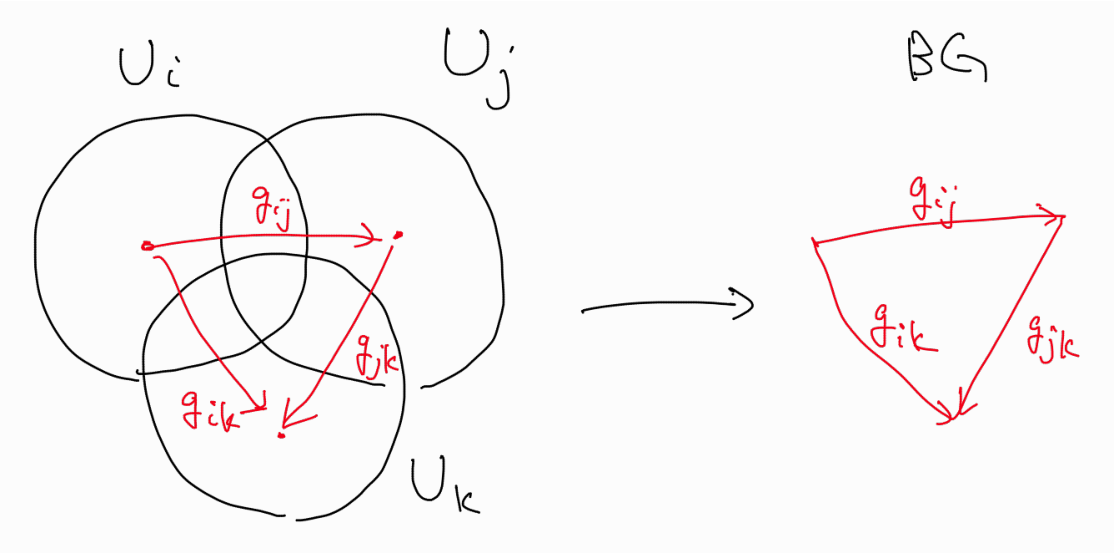
\includegraphics[width=0.62\textwidth]{figures/fig9_1.png}\\[2pt]
  {\small 图 9.1：由卡与到 $BG$ 的映射定义的主 $G$-丛。}
\end{center}

\takeaway{分类空间可以造得很具体：$EG$ 是单纯复形，其单形取自群元素的元组，$G$ 的左乘作用自由、$EG$ 可缩；商空间 $BG=EG/G$ 的 $n$-单形记作 $(g_1|\cdots|g_n)$。反之，$M$ 上主 $G$-丛对应的映射 $M\to BG$ 只是把粘贴元 $g_{ij}$ 编码成拓扑数据。}

\section{$BG$ 的单纯上同调}

利用边缘映射 (9.4)，我们可以容易地写下 $BG$ 以阿贝尔群 $A$ 为系数的单纯上同调的定义。$k$-上链就是函数
\begin{equation}
  f(g_1,g_2,\dots,g_k)\in A,
  \tag{9.5}
\end{equation}

% [原文 p.132]
而上边缘映射为
\begin{equation}
  \begin{aligned}
    (\delta f)(g_1,g_2,\dots,g_k,g_{k+1})={}&f(g_2,\dots,g_k,g_{k+1})-f(g_1g_2,g_3,\dots,g_{k+1})\\
    &+f(g_1,g_2g_3,\dots,g_{k+1})+\cdots\\
    &+(-1)^k f(g_1,\dots,g_{k-1},g_kg_{k+1})+(-1)^{k+1}f(g_1,\dots,g_k).
  \end{aligned}
  \tag{9.6}
\end{equation}

由此我们理解了 $H^k(BG;A)$ 的定义。这里我们利用 $BG$ 的显式构造，自然地写下了与有限群 $G$ 相伴的这些上同调群的定义。同一定义也可以纯代数地得到；在后一种语境中，所得的上同调群称为 $G$ 的群上同调，并（颇易混淆地）记作 $H^k(G;A)$。它不同于把 $G$ 看作带离散拓扑的拓扑空间时定义的 $H^k(G;A)$。本系列讲义坚持前一种记号，但读者应知道，后一种记号在文献中也广泛使用。

具体地，对 1-上链 $f(g_1)$，
\begin{equation}
  (\delta f)(g_1,g_2)=f(g_2)-f(g_1g_2)+f(g_1).
  \tag{9.7}
\end{equation}
因此 $\delta f=0$ 意味着 $f$ 是 $G\to A$ 的同态。对 2-上链 $f(g_1,g_2)$，
\begin{equation}
  (\delta f)(g_1,g_2,g_3)=f(g_2,g_3)-f(g_1g_2,g_3)+f(g_1,g_2g_3)-f(g_1,g_2).
  \tag{9.8}
\end{equation}
对 3-上链 $f(g_1,g_2,g_3)$，
\begin{equation}
  \begin{aligned}
    (\delta f)(g_1,g_2,g_3,g_4)={}&f(g_2,g_3,g_4)-f(g_1g_2,g_3,g_4)\\
    &+f(g_1,g_2g_3,g_4)-f(g_1,g_2,g_3g_4)+f(g_1,g_2,g_3).
  \end{aligned}
  \tag{9.9}
\end{equation}

我们来看看这些表达式如何在其他语境中自然地出现。

\takeaway{$BG$ 的单纯上同调可直接用边缘映射 (9.4) 写出：$k$-上链是函数 $f(g_1,\dots,g_k)\in A$，上边缘由式 (9.6) 给出。同一构造从纯代数角度给出 $G$ 的群上同调，写作 $H^k(G;A)$；式 (9.7)–(9.9) 分别是 1、2、3-上链的显式公式。}

\section{$H^2$ 与群扩张}

\subsection{基本设定}

考虑群的正合列
\begin{equation}
  1\to A\to\Gamma\to G\to 1,
  \tag{9.10}
\end{equation}
$\Gamma$ 称为 $G$ 被 $A$ 的一个扩张。

为简单起见，设 $A$ 在 $\Gamma$ 的中心，即对所有 $\gamma\in\Gamma$ 有 $\gamma a=a\gamma$。这样的扩张称为中心扩张。这特别意味着 $A$ 是阿贝尔群。注意我们对群运算使用乘法记号，包括 $A$ 的运算。

我们希望用 $G$ 与 $A$ 描述 $\Gamma$。为此，对每个 $g\in G$ 取一个代表元 $\gamma_g\in\Gamma$。于是 $\Gamma$ 的任一元素可写成 $a\gamma_g$，其中 $g\in G$，$a\in A$。现在 $\gamma_g\gamma_h$ 映到 $gh\in G$，因此存在元素 $a(g,h)\in A$ 使
\begin{equation}
  \gamma_g\gamma_h=a(g,h)\gamma_{gh}.
  \tag{9.11}
\end{equation}

% [原文 p.133]
这个 $a(g,h)$ 是 2-上链，并且不难发现它是 2-上闭链。

为看出这一点，我们用两种方式计算 $\gamma_g\gamma_h\gamma_k$：一方面
\begin{equation}
  \gamma_g\gamma_h\gamma_k=a(g,h)\gamma_{gh}\gamma_k=a(g,h)a(gh,k)\gamma_{ghk},
  \tag{9.12}
\end{equation}
另一方面
\begin{equation}
  \gamma_g\gamma_h\gamma_k=a(h,k)\gamma_g\gamma_{hk}=a(g,hk)a(h,k)\gamma_{ghk},
  \tag{9.13}
\end{equation}
于是
\begin{equation}
  a(g,h)a(gh,k)=a(g,hk)a(h,k),
  \tag{9.14}
\end{equation}
这正是式 (9.8) 中的 $\delta a=0$ 的乘法写法。

我们还要注意 $\gamma_g$ 的选取不唯一：同样可以取 $\tilde\gamma_g:=\gamma_gb(g)$，其中 $b(g)\in A$。此时
\[
  \tilde\gamma_g\tilde\gamma_h=\tilde a(g,h)\tilde\gamma_{gh},
\]
其中
\begin{equation}
  \tilde a(g,h)=\frac{b(g)b(h)}{b(gh)}a(g,h),
  \tag{9.15}
\end{equation}
这正是式 (9.7) 中的 $\tilde a=a+\delta b$ 的乘法写法。
% [Tutor Note: 原文此处作 “for any a ∈ A”，按上下文应为 b(g) ∈ A；式 (9.15) 的分母原文印作 g(gh)，应为 b(gh)。两处均按最合理读法译出，已登记进原文笔误表。]

因此我们看到，中心扩张 (9.10) 由第二上同调群 $H^2(BG;A)$ 分类。

\subsection{小学就学过的例子}

我们小学就见过这个例子。（这一点在许多地方被指出过，但我不记得最初是在哪里学到的。例如可在 [Isa02] 中找到，那是一位代数拓扑学家所写。）

考虑扩张
\begin{equation}
  0\to\Z_{10}\to\Z_{100}\to\Z_{10}\to 0,
  \tag{9.16}
\end{equation}
其中群运算用加法记号，映射 $\Z_{10}\to\Z_{100}$ 由乘 10 给出，映射 $\Z_{100}\to\Z_{10}$ 由模 10 给出。于是 $\Z_{100}$ 的每个元素可写成 $(a,g)$，其中 $a\in\Z_{10}$，$g\in\Z_{10}$，加法法则为
\begin{equation}
  (a_1,g_1)+(a_2,g_2)=(a_1+a_2+a(g_1,g_2),\,g_1+g_2),
  \tag{9.17}
\end{equation}
其中
\begin{equation}
  a(g_1,g_2)=
  \begin{cases}
    0 & g_1+g_2<10,\\
    1 & g_1+g_2\ge 10.
  \end{cases}
  \tag{9.18}
\end{equation}

这是 2-上闭链（你验证过吗？），它定义了 $H^2(B\Z_{10};\Z_{10})$ 的一个非平凡元素。

这个重要的函数 $a(g_1,g_2)$ 在日语中称为“繰り上がり”，英语中称为 carry（进位）。

% [原文 p.134]
\subsection{量子力学中的射影表示}

在量子力学中，群 $G$ 作用在希尔伯特空间 $\mathcal H$ 上。最直接地，它由满足
\begin{equation}
  U(g_1)U(g_2)=U(g_1g_2)
  \tag{9.19}
\end{equation}
的 $G$ 的表示给出。话虽如此，由于物理只关心 $\mathcal H$ 中元素 $v$ 到相差一个相位的程度，我们可以把这个要求减弱为
\begin{equation}
  U(g_1)U(g_2)=\alpha(g_1,g_2)U(g_1g_2),
  \tag{9.20}
\end{equation}
其中 $\alpha(g_1,g_2)\in U(1)=\{z\mid |z|=1\}$。这称为 $G$ 的射影表示，$\alpha(g_1,g_2)$ 称为射影相位。用与上面相同的论证可知，$\alpha(g_1,g_2)$ 是 2-上闭链；把 $U(g)$ 换成 $U(g)b(g)$，其中 $b(g)\in U(1)$，会把 $\alpha(g_1,g_2)$ 换成与之上同调的 $\tilde\alpha(g_1,g_2)$。因此，射影表示的类型由 $H^2(BG;U(1))$ 中的一个类指定。

此时，对称操作后的态矢量会相差一个相位，这取决于我们是一次作用 $gh$，还是先后作用 $g$ 与 $h$。对称性没有以最标准、最朴素的方式实现。但这一非标准实现仍受上闭链条件的约束。

在 hep-th 中，我们常考虑配分函数而不是态矢量。在量子力学情形，考虑插入对称作用的热配分函数。当对称作用是射影的，我们有
\begin{equation}
  \tr e^{-\beta H}U(g)U(h)=\alpha(g,h)\tr e^{-\beta H}U(gh).
  \tag{9.21}
\end{equation}
这是周长为 $\beta$ 的 $S^1$ 上的配分函数，其上带有一个和乐（holonomy）为 $gh$ 的 $G$-丛。取决于如何表示这个 $G$-丛——用一个粘贴处 $gh$，还是用两个粘贴处分别取 $g$ 与 $h$——我们得到略有不同的配分函数，其差别只是一个相位，且受上闭链条件约束。

把量子力学系统看作 0+1 维系统，这个射影相位是（量子）反常最简单的例子，它可以理解为来自体的流入。为此，我们需要学习 1+1 维可逆拓扑相最基本的情形。

\subsection{$H^2$ 与 1+1 维的可逆拓扑相}

考虑带三角剖分的 2 维流形 $M$，其上带有主 $G$-丛。这给出映射 $f\colon M\to BG$。现在选取一个上同调类 $\alpha\in H^2(BG;U(1))$，其中我们把 $U(1)\simeq\R/\Z$ 并使用加法记号。用 $f$ 拉回 $\alpha$，得到类 $f^*(\alpha)\in H^2(M;U(1))$。可以在 $M$ 上积分它，得到一个值 $\int_Mf^*(\alpha)\in\R/\Z$。于是可以考虑一个（相当平凡的）1+1 维系统，其配分函数为
\begin{equation}
  \exp\Bigl(2\pi i\int_M f^*(\alpha)\Bigr).
  \tag{9.22}
\end{equation}

% [原文 p.135]
如果展开并还原定义，这不过意味着我们计算
\begin{equation}
  \exp\Bigl(2\pi i\sum_{\text{$M$ 的三角形 }(ijk)}\alpha(g_{ij},g_{jk})\Bigr).
  \tag{9.23}
\end{equation}

\begin{center}
  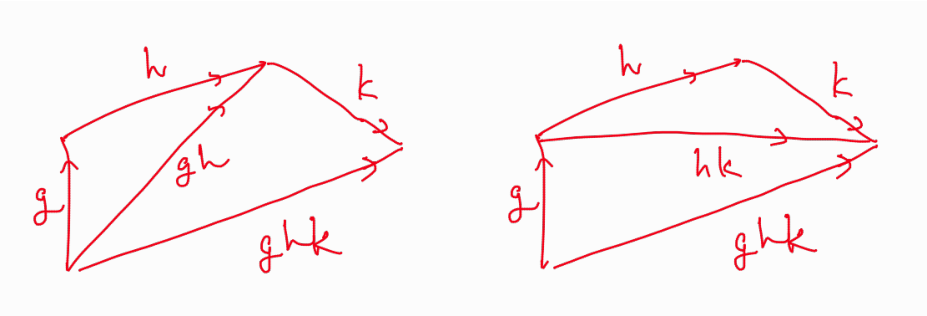
\includegraphics[width=0.62\textwidth]{figures/fig9_2.png}\\[2pt]
  {\small 图 9.2：矩形的两种三角剖分。}
\end{center}
这个值与我们在流形上放置的三角剖分无关。例如，考虑图 9.2 所示的同一矩形的两种局部构型。对左边的构型，我们得到局部因子
\begin{equation}
  \alpha(g,h)+\alpha(gh,k),
  \tag{9.24}
\end{equation}
对右边的构型类似地得到
\begin{equation}
  \alpha(g,hk)+\alpha(h,k).
  \tag{9.25}
\end{equation}
上面两式相等正是条件 $\delta\alpha=0$，即 (9.8) 给出的条件。


这个构造最初由 [DW90] 引入物理，尽管那篇论文对所有可能的 $G$-丛求和（所以它是有限群规范理论）。这里我们把 $G$-丛保持为背景场的一部分。这个可逆相常称为 Dijkgraaf--Witten 相。

这是可逆拓扑相最简单的非平凡例子。这个名字背后有各种理由，其中之一是配分函数的值总不为零，因而可逆。它也是 $G$-对称保护拓扑（SPT）相的一个例子。

\subsection{反常流入}

现在考虑这个 1+1 维系统有 0+1 维边界的情形，见图 9.3。图里我们还画出了三角剖分的对偶图；对偶边可看作相应的 $G$ 变换发生的地方。对偶边常称为拓扑 $G$ 畴壁。在边界上，这些畴壁对边界希尔伯特空间有相应作用。在左边，我们有先后作用 $U(g)$ 与 $U(h)$。在右边，我们有单次作用 $U(gh)$。在左边，我们还多一个三角形，给出额外相位 $\exp(2\pi i\alpha(g,h))$。为使两边的配分函数一致，我们看到需要
\begin{equation}
  U(g)U(h)\exp(2\pi i\alpha(g,h))=U(gh),
  \tag{9.26}
\end{equation}

% [原文 p.136]
\begin{center}
  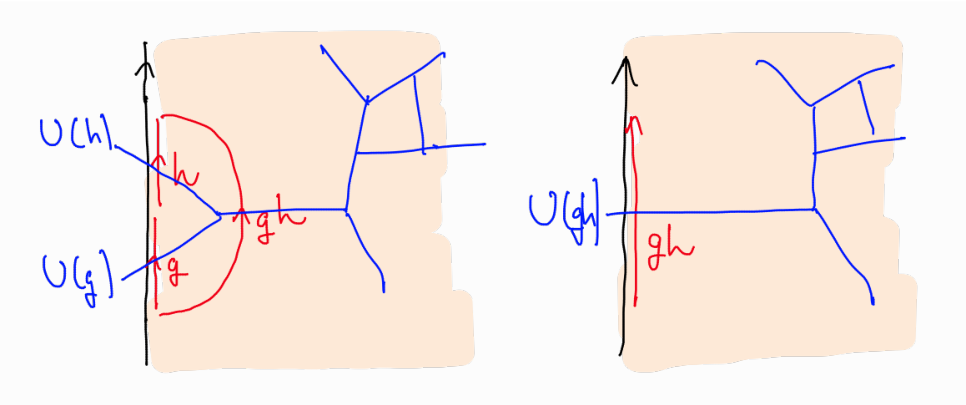
\includegraphics[width=0.62\textwidth]{figures/fig9_3.png}\\[2pt]
  {\small 图 9.3：1+1 维 Dijkgraaf--Witten 理论的边界。}
\end{center}

\begin{center}
  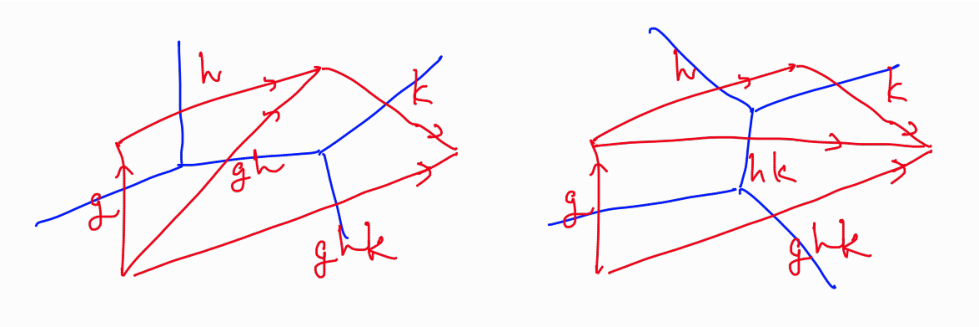
\includegraphics[width=0.62\textwidth]{figures/fig9_4.png}\\[2pt]
  {\small 图 9.4：在 1+1 维中重构 $G$ 畴壁。}
\end{center}

也就是说，边界希尔伯特空间上的 $G$ 作用是射影的，其射影相位由体可逆 Dijkgraaf--Witten 相的选取固定。

我们最初讨论射影对称作用时，把 $\alpha(g,h)$ 看成一个可能恼人的额外相位，它显示对称作用的结果有轻微的不唯一性，或者说等价于系统有量子反常。引入体可逆相之后，这种不唯一性恰恰是所需要的：它使 0+1 维边界与 1+1 维体组成的总系统不依赖于我们决定怎样作用 $gh$——是一次作用，还是先后作用 $g$ 再作用 $h$。我们说存在来自体的反常流入。我们也说存在体--边对应，即体的拓扑性质决定边界的反常。

\takeaway{中心扩张由 2-上闭链 $a(g,h)$ 描写，改选代表元对应 $a\mapsto a+\delta b$，故扩张由 $H^2(BG;A)$ 分类。同一上同调控制量子力学射影表示的相位与 1+1 维 Dijkgraaf--Witten 可逆相：边界的射影相位由体相固定，这就是最简单的反常流入。}

\section{$H^3$ 与 1+1 维系统的反常}

到目前为止，我们讨论了 0+1 维的射影作用（即反常）以及对应的 1+1 维可逆相，它们都由 $H^2$ 控制。现在讨论 1+1 维的反常与对应的 2+1 维可逆相。我们将看到，它们由 $H^3$ 控制。

\subsection{1+1 维的反常与来自 2+1 维的流入}

现在考虑 1+1 维中的 $G$-畴壁。图 9.4 给出了图示，我们也画出了对偶三角剖分。我们不再要求两侧给出相同结果；相反，我们假定从左到右的重构会产生一个相位。让我们用 $(gh)k$ 示意地记左边的构型，用 $g(hk)$ 记右边的构型，并假定它们相差一个相位 $\omega$：
% [Tutor Note: 原文此句作 “related by a phase α”，但紧随的式 (9.27) 及后文一律用 ω；按最合理读法译作 ω，已登记进原文笔误表。]

% [原文 p.137]
\begin{equation}
  Z_{(gh)k}=\exp(2\pi i\omega(g,h,k))Z_{g(hk)}.
  \tag{9.27}
\end{equation}

现在考虑四个畴壁 $g_{1,2,3,4}$ 连接成墙 $g_1g_2g_3g_4$。我们可以改变连接方式，一种方式是
\begin{equation}
  g_1(g_2(g_3g_4))\to g_1((g_2g_3)g_4)\to(g_1(g_2g_3))g_4\to((g_1g_2)g_3)g_4,
  \tag{9.28}
\end{equation}
另一种方式是
\begin{equation}
  g_1(g_2(g_3g_4))\to(g_1g_2)(g_3g_4)\to((g_1g_2)g_3)g_4.
  \tag{9.29}
\end{equation}
这两种过程的一致性要求条件
\begin{equation}
  \omega(g_2,g_3,g_4)+\omega(g_1,g_2g_3,g_4)+\omega(g_1,g_2,g_3)
  =\omega(g_1,g_2,g_3g_4)+\omega(g_1g_2,g_3,g_4),
  \tag{9.30}
\end{equation}
这正是式 (9.9) 给出的 $\delta\omega=0$。因此它是 3-上闭链，确定一个类 $\omega\in H^3(BG;U(1))$。

\begin{center}
  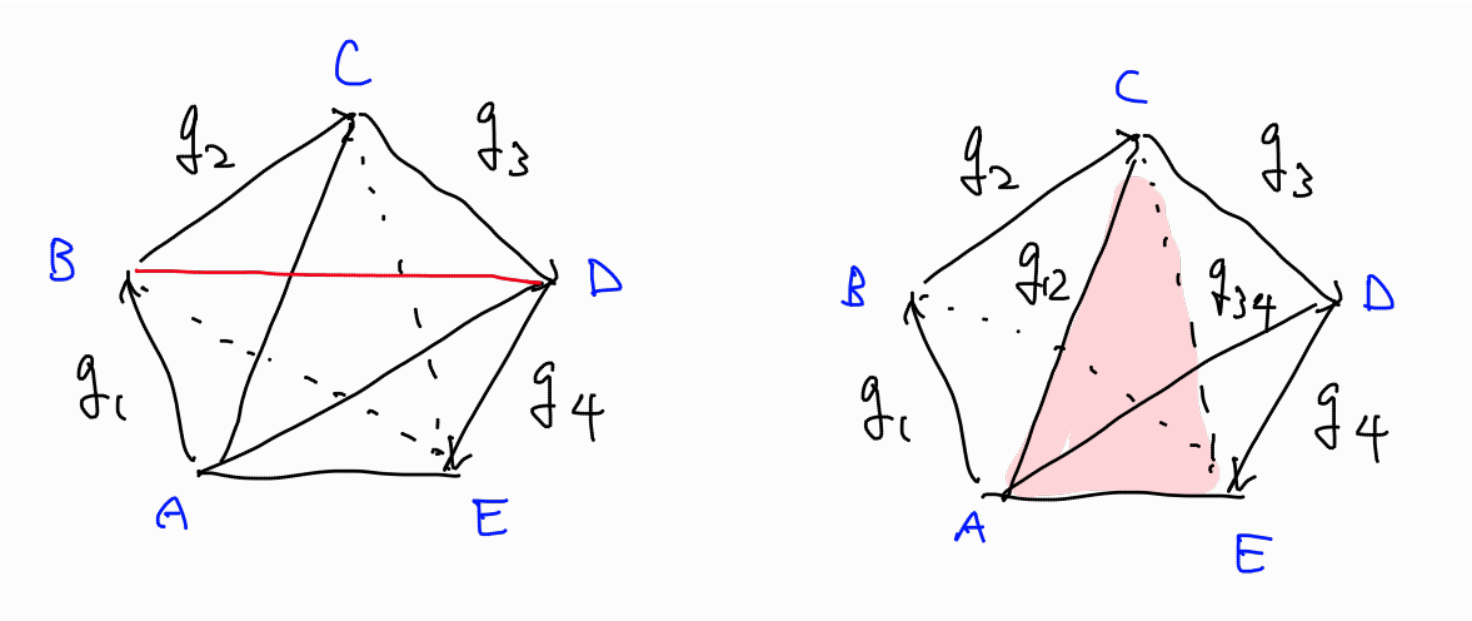
\includegraphics[width=0.62\textwidth]{figures/fig9_5.png}\\[2pt]
  {\small 图 9.5：两种局部构型。左：三个四面体；右：两个四面体。}
\end{center}

注意同一个类 $\omega$ 如法定义了 2+1 维的可逆拓扑相；在带有由 $f\colon M_3\to BG$ 给出的 $G$-丛的流形 $M_3$ 上，配分函数简单地由
\begin{equation}
  \exp\Bigl(2\pi i\int_{M_3}f^*(\omega)\Bigr)
  =\exp\Bigl(2\pi i\sum_{\text{四面体 }(ijkl)}\omega(g_{ij},g_{jk},g_{kl})\Bigr)
  \tag{9.31}
\end{equation}
给出。这一次，三角剖分选取改变下的不变性例如由图 9.5 中的局部移动保证。在左边，我们有三个共边 $BD$ 的四面体，即 $ABCD$、$ABDE$ 与 $BCDE$。在右边，我们有两个共面 $ACE$ 的四面体，即 $ABCE$ 与 $ACDE$。令两边的局部贡献相等，就得到式 (9.30)。

现在可以把此可逆 Dijkgraaf--Witten 相贴到边界上，使相位 (9.27) 由体中的一个额外单形提供，见图 9.6。与之前一样，边界--体复合系统在三角剖分改变下不变。

% [原文 p.138]
\begin{center}
  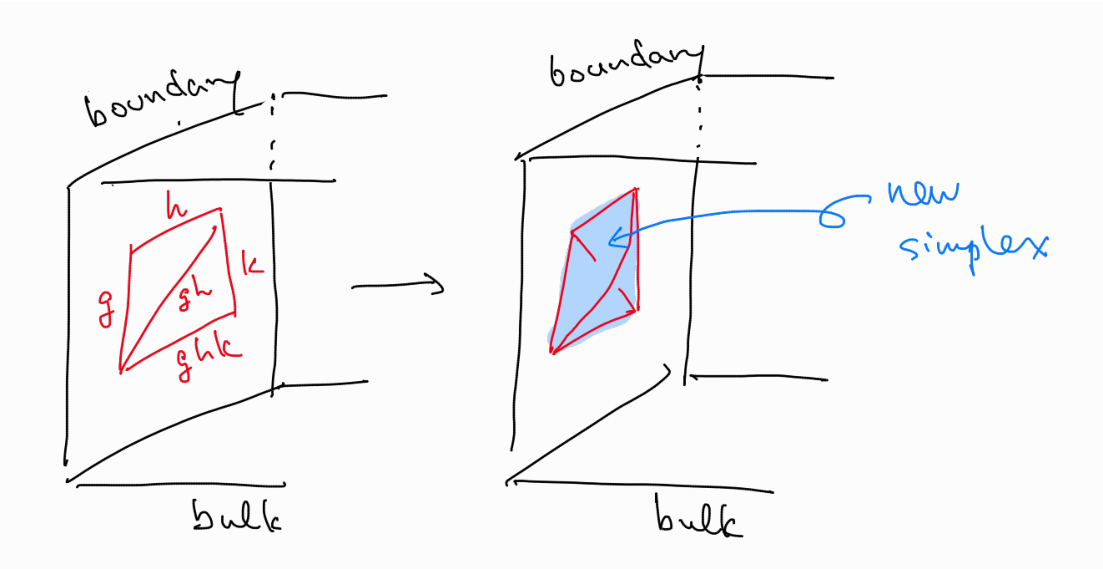
\includegraphics[width=0.62\textwidth]{figures/fig9_6.png}\\[2pt]
  {\small 图 9.6：从 2+1 维到 1+1 维的反常流入。}
\end{center}

\subsection{反常的“哈密顿量”定义}

到目前为止，我们对 1+1 维中有限群对称性的反常已有相当好的理解。但我们能写下具有这种对称性的显式系统吗？0+1 维中对应的问题很容易：随便取一个射影表示即可。1+1 维中有类似的显式构造吗？图 9.4 与式 (9.27) 在那个显式语境中意味着什么？

让我们先把式 (9.27) 变得更具体。这在 AQFT 中由 [Mug04, Sec.~4.2] 完成（虽然更早就已知道；只是我找不到更早的文献），在 cond-mat 中由 [EN14] 完成，在 hep-th 中由 [Sei23] 完成。文献中最常见的名称似乎是 Else--Nayak 论证。

设 $\mathcal H_{g,h}$ 是一个 $g$-壁与一个 $h$-壁上的希尔伯特空间。设 $\mathcal H_g$ 是某处单个 $gh$-壁上的希尔伯特空间。应当存在一个酉算子 $u(g,h)\colon\mathcal H_{g,h}\to\mathcal H_g$，局域地支撑在交点附近，见图 9.7。

\begin{center}
  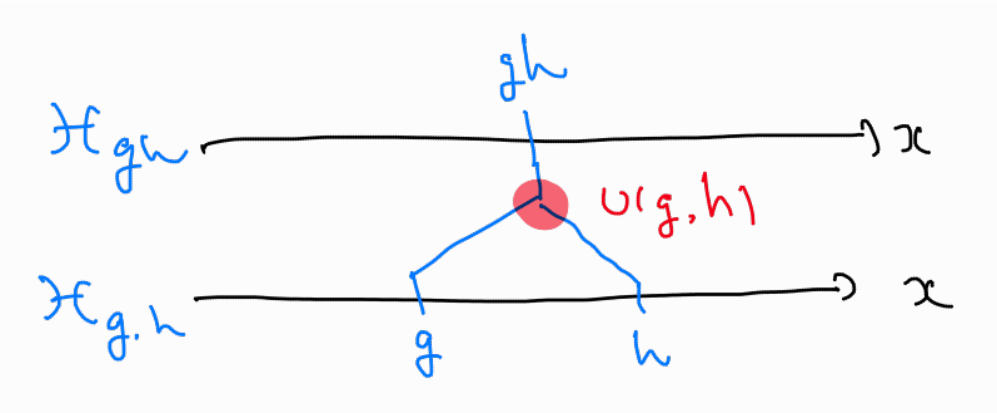
\includegraphics[width=0.62\textwidth]{figures/fig9_7.png}\\[2pt]
  {\small 图 9.7：两个壁的交点酉算子 $u(g,h)$。}
\end{center}

为了进一步用更基本的成分改写 $u(g,h)$，考虑在半空间上施加群变换，如图 9.9 所示：
\begin{equation}
  U_g\colon\mathcal H\to\mathcal H_g.
  \tag{9.32}
\end{equation}
于是我们可以说
\begin{equation}
  U_gU_h\propto u(g,h)U_{gh}.
  \tag{9.33}
\end{equation}

% [原文 p.139]
\begin{center}
  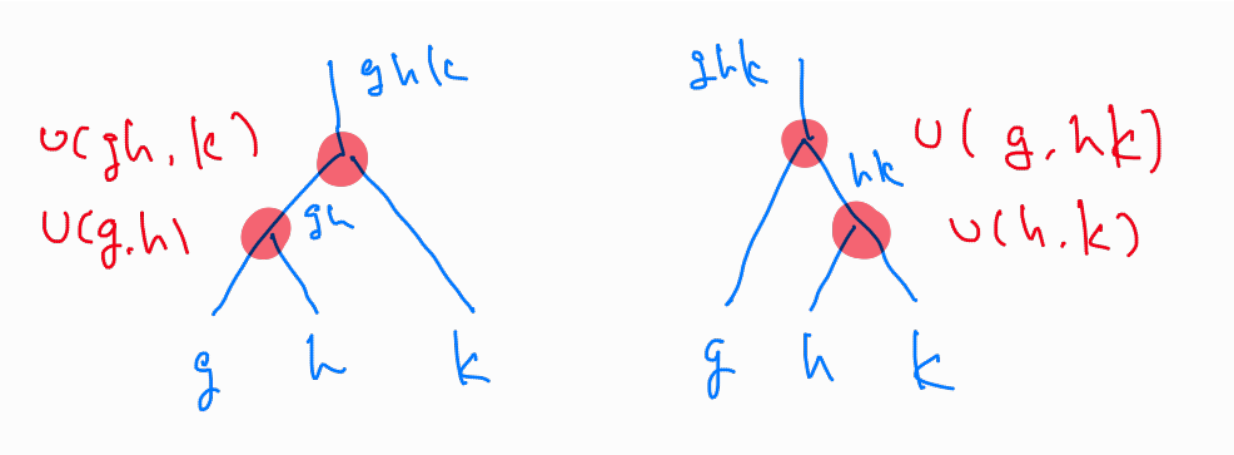
\includegraphics[width=0.62\textwidth]{figures/fig9_8.png}\\[2pt]
  {\small 图 9.8：结合三个壁的两种方式。}
\end{center}

\begin{center}
  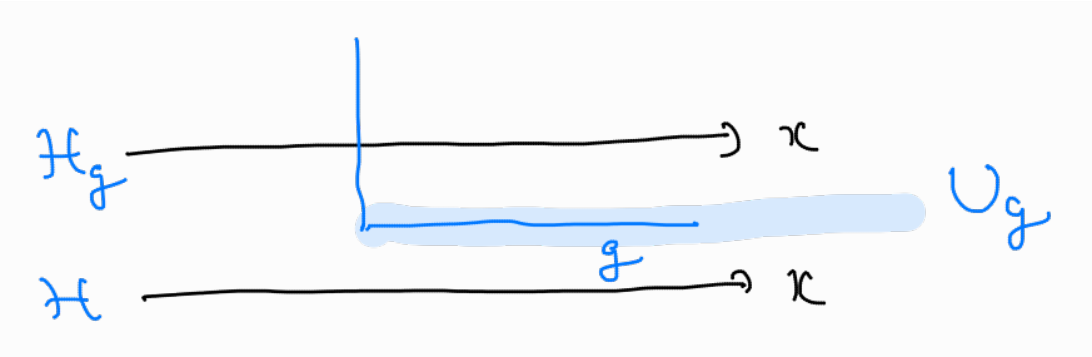
\includegraphics[width=0.62\textwidth]{figures/fig9_9.png}\\[2pt]
  {\small 图 9.9：半空间上的群变换。}
\end{center}

这里 $u(g,h)$ 只定义到相差一个相位，因为像 $U_g$ 这样的整体作用酉算子，只定义为对局域算子 $O$ 的作用 $O\mapsto U_gOU_g^{-1}$，其相位部分没有良定义。

现在我们考虑融合三个壁的过程。有两种方式，如图 9.8 所示。注意这个图与图 9.4 相同，只是从侧面看。研究如何以两种不同次序把 $U_gU_hU_k$ 改写成 $U_{ghk}$，并记住 $U_g$ 等都只定义到相差一个相位，我们发现
\begin{equation}
  (U_gu(h,k)U_g^{-1})u(g,hk)=e^{2\pi i\omega(g,h,k)}u(g,h)u(gh,k).
  \tag{9.34}
\end{equation}
这可以看作式 (9.27) 更显式的版本。

总结一下：我们考虑“整体”操作 $U_g$，它作用的“射影性”（即 1-上闭链条件失效）不用复相位表示，而用局域酉算子 $u(g,h)$ 表示。后者又在 2-上闭链条件上失效，如式 (9.34) 所示，这就给出我们想要的相位 $\omega(g,h,k)$。确实可以由式 (9.34) 经一个略长但直接的计算证明 $\omega(g,h,k)$ 是 3-上闭链。

\subsection{显式自旋链模型}

作为一个显式例子，考虑一个“自旋链”：每个格点的局域希尔伯特空间是 $\C^{|G|}$，由 $g\in G$ 的 $\ket{g}$ 张成。链的一个态是 $\ket{\cdots g_ig_{i+1}g_{i+2}\cdots}$。让 $g\in G$ 如下作用在链上：
\begin{equation}
  \ket{\cdots g_ig_{i+1}g_{i+2}\cdots}
  \mapsto\prod_i e^{2\pi i\alpha(g,\,g_{i+1},\,g_{i+1}^{-1}g_i)}
  \ket{\cdots gg_i,gg_{i+1},gg_{i+2},\cdots},
  \tag{9.35}
\end{equation}

% [原文 p.140]
其中 $\alpha$ 是 3-上闭链。

我们的目标是依次构造 $U_g$、$u(g,h)$ 与 $\omega(g,h,k)$，证明这个系统的反常是 $\omega=-\alpha$。为确定起见，令 $U_g$ 为同一作用限制在格点 $i_L<i<i_R$ 上。于是由 $\omega$ 的上闭链条件，我们得到
\begin{equation}
  U_gU_h=U_{gh}e^{2\pi i\omega(g,h,g_{i_L})}e^{-2\pi i\omega(g,h,g_{i_R})}.
  \tag{9.36}
\end{equation}
注意我们不能令 $i_R\to\infty$，然后说 $U_g$ 连同相位都良定义。但若你接受 $U_g$ 只定义到相差一个相位，就可以令 $i_R\to\infty$，且
\begin{equation}
  u(g,h)\ket{ghk}=e^{2\pi i\omega(g,h,k)}\ket{ghk}.
  \tag{9.37}
\end{equation}
% [Tutor Note: 式 (9.37) 原文指数印作 e^{2πω(g,h,k)}，缺因子 i；按上下文（相位须为模 1 的复数）补为 e^{2πiω}，已登记进原文笔误表。]

现在我们研究式 (9.34) 两边对 $\ket{ghk\ell}$ 的作用。我们发现
\begin{equation}
  \alpha(h,k,\ell)+\alpha(g,hk,\ell)
  =\omega(g,h,k)+\alpha(g,h,k\ell)+\alpha(gh,k,\ell),
  \tag{9.38}
\end{equation}
也就是说
\begin{equation}
  \omega=-\alpha.
  \tag{9.39}
\end{equation}

例如，考虑 $G=\Z_2=\{0,1\}$。此时 $H^3(BG,U(1))=\Z_2$。非平凡的上闭链取为
\begin{equation}
  \begin{cases}
    e^{2\pi i\alpha(1,1,1)}=-1,\\
    e^{2\pi i\alpha(a,b,c)}=+1 & \text{若 } a,b,c \text{ 中任一为零}.
  \end{cases}
  \tag{9.40}
\end{equation}
% [Tutor Note: 式 (9.40) 原文指数亦印作 e^{2πα}，缺因子 i，同样按最合理读法补上，已登记进原文笔误表。]

则 $\Z_2$ 作用是各 $X_i$（交换 $\ket{0}$ 与 $\ket{1}$）之积，再按式 (9.35) 加上额外相位，即它对两个相邻格点作用为
\begin{equation}
  \ket{00}\mapsto+\ket{11},\quad
  \ket{01}\mapsto+\ket{10},\quad
  \ket{10}\mapsto+\ket{01},\quad
  \ket{11}\mapsto-\ket{00}.
  \tag{9.41}
\end{equation}

要写下具有任意反常 $\omega$ 的有限群 $G$ 的显式 1 维自旋链模型，我们任取一个支撑在格点 $i$ 附近的有限程局域算子 $O_i$。然后对它按群作用取平均，再设 $H=\sum_iO_i$。这是平移不变的，且是有限程的。用这种方式对上述反常 $\Z_2$ 得到的一个具体哈密顿量为\footnote{2021 年 12 月，在与 Yunqin Zheng 与 Philip Boyle Smith 的一次未发表合作中，我们出于这个动机开始研究这个模型。做过一些数值计算后，我们注意到它的长程极限应当是一个 $c=1$ 的 CFT。我们问 Katsura 先生是否在文献中见过这个模型，他说经 Kramers--Wannier 变换后，它是某个特殊参数值下的 Ashkin--Teller 模型。有个博学的朋友真好。}
\begin{equation}
  H=-\sum_i(Z_{i-1}X_i+Z_{i-1}Z_{i+1}+X_iZ_{i+1}).
  \tag{9.42}
\end{equation}

\takeaway{1+1 维中畴壁的重构产生相位 $\omega(g,h,k)$，四个壁结合的两种方式给出 $\delta\omega=0$，故 $\omega\in H^3(BG;U(1))$，它定义 2+1 维可逆相并向边界流入反常。显式模型中整体算子 $U_g$ 的射影性由局域酉算子 $u(g,h)$ 承担，自旋链的反常为 $\omega=-\alpha$。}

% [原文 p.141]
\section{计算 $H^k(BG;U(1))$}

一般这很难。当 $G=\Z_n$ 时，
\begin{equation}
  H^k(B\Z_n;U(1))=
  \begin{cases}
    U(1) & k=0,\\
    \Z_n & k=1,3,5,\dots,\\
    0 & k=2,4,6,\dots.
  \end{cases}
  \tag{9.43}
\end{equation}
$k=1$ 的结果是直接的，因为 $H^1(BG;U(1))$ 的元素正是 $G\to U(1)$ 的同态。$k=3$ 的显式上闭链由
\begin{equation}
  \alpha(a,b,c)=\tfrac1n p(a,b)c \bmod 1
  \tag{9.44}
\end{equation}
给出，其中 $a,b,c\in\{0,\dots,n-1\}$，而 $p(a,b)$ 是进位（日语“繰り上がり”，英语 the carry）：
\begin{equation}
  p(a,b)=
  \begin{cases}
    0 & a+b<n,\\
    1 & a+b\ge n.
  \end{cases}
  \tag{9.45}
\end{equation}

对于小的群 $G$，可以直接用 GAP（一个由数学家编写的开源计算机代数系统，面向群与代数），或用 SAGE（一个基于 python 的系统，包装了不同子领域的数学家编写的多个计算机代数系统）。GAP 的 HAP 包有函数 \texttt{GroupHomology}，可计算 $H_k(BG;\Z)$；由此经万有系数定理可计算任意 $A$ 的 $H^k(BG;A)$。特别地，$H^k(BG;U(1))$ 就是 $H_k(BG;\Z)$ 的 Pontryagin 对偶（到 $U(1)$ 的同态群）。还有专有系统 Magma（同样由数学家编写、面向群与代数），我没用过，听说它比 GAP 略好一些。

对于大的有限群，这就不平凡了。例如 Monster 群 $M$（最大的散在有限单群），$H^3(BM;U(1))$ 尚未确定，猜想是 $\Z_{24}$；至少已知 Monster CFT 反常 $\omega$ 的阶为 24，因此 $H^3(BM;U(1))$ 包含 $\Z_{24}$ [JF17]。

\takeaway{$H^k(BG;U(1))$ 一般难算。$G=\Z_n$ 时结果由式 (9.43) 给出，$k=3$ 的上闭链是式 (9.44)。小群可用 GAP 的 HAP 包算 $H_k(BG;\Z)$，再经万有系数定理与 Pontryagin 对偶得到；大群如 Monster 群仍未知，猜想 $H^3(BM;U(1))=\Z_{24}$。}

\chapterreview{本章以有限群 $G$ 的分类空间 $BG$ 为例，说明如何手工造出 $EG$ 这个可缩主丛，并把 $M$ 上主丛的粘贴数据编码成映射 $M\to BG$。由此得到 $BG$ 的单纯上同调，它与纯代数定义的群上同调一致。$H^2$ 部分讲中心扩张、射影表示与 1+1 维 Dijkgraaf--Witten 相，并说明边界射影相位由体相决定，此即反常流入。$H^3$ 部分把同样思路推广到 1+1 维反常与 2+1 维可逆相，并以显式自旋链模型算出 $\omega=-\alpha$。最后交代 $\Z_n$ 情形的结果与 GAP 等计算工具，指出大群情形仍无一般答案。}
